\let\negmedspace\undefined
\let\negthickspace\undefined
\documentclass[journal,12pt,onecolumn]{IEEEtran}
\usepackage{cite}
\usepackage{amsmath,amssymb,amsfonts,amsthm}
\usepackage{algorithmic}
\usepackage{graphicx}
\graphicspath{{Figs/}}
\usepackage{textcomp}
\usepackage{xcolor}
\usepackage{txfonts}
\usepackage{listings}
\usepackage{enumitem}
\usepackage{mathtools}
\usepackage{gensymb}
\usepackage{comment}
\usepackage{caption}
\usepackage[breaklinks=true]{hyperref}
\usepackage{tkz-euclide} 
\usepackage{listings}
\usepackage{gvv}                                        
%\def\inputGnumericTable{}                                 
\usepackage[latin1]{inputenc}     
\usepackage{xparse}
\usepackage{color}                                            
\usepackage{array}                                            
\usepackage{longtable}                                       
\usepackage{calc}                                             
\usepackage{multirow}
\usepackage{multicol}
\usepackage{hhline}                                           
\usepackage{ifthen}                                           
\usepackage{lscape}
\usepackage{tabularx}
\usepackage{array}
\usepackage{float}
%\newtheorem{theorem}{Theorem}[section]
%\newtheorem{theorem}{Theorem}[section]
%\newtheorem{problem}{Problem}
%\newtheorem{proposition}{Proposition}[section]
%\newtheorem{lemma}{Lemma}[section]
%\newtheorem{corollary}[theorem]{Corollary}
%\newtheorem{example}{Example}[section]
%\newtheorem{definition}[problem]{Definition}

\begin{document}


\title{4.13.71}
\author{AI25BTECH11002 - Ayush Sunil Labhade}
{\let\newpage\relax\maketitle}


\textbf{Question:}

If the vectors \(a \hat{i} + \hat{j} + \hat{k}\), \(\hat{i} + b \hat{j} + \hat{k}\) and \(\hat{i} + \hat{j} + c \hat{k}\) \((a \neq b \neq c \neq 1)\) are co-planar, then
the value of \(\dfrac{1}{1-a} + \dfrac{1}{1-b} + \dfrac{1}{1-c} = \dotsb\).

\textbf{Solution:}

The vectors are coplanar if they are linearly dependent, i.e., the matrix formed by them has rank less than 3.

Let \(\vec{u} = a \hat{i} + \hat{j} + \hat{k}\), \(\vec{v} = \hat{i} + b \hat{j} + \hat{k}\), \(\vec{w} = \hat{i} + \hat{j} + c \hat{k}\).

Form the matrix
\begin{align}
	\vec{M} = \myvec{a & 1 & 1 \\ 1 & b & 1 \\ 1 & 1 & c}.
\end{align}

For rank $<3$, perform row reduction to find the condition.

After row reducing the matrix:

\begin{align}
\myvec{1 & b & 1 \\ 0 & 1 - ab & 1 - a \\ 0 & 1 - b & c - 1}.
\end{align}

Assuming \(1 - ab \neq 0\) (consistent with \(a \neq b \neq 1\)), to eliminate the second column in $R_3$, compute the multiplier \(k = \frac{1 - b}{1 - ab}\).

Replace $R_3$ with $R_3$ $-$ \(k\) $R_2$:

The second entry becomes \(1 - b - k (1 - ab) = 0\) by construction.
The third entry becomes \(c - 1 - k (1 - a) = 0\) for the row to be zero (ensuring rank 2).

For rank $<3$, the third entry must be zero:
\begin{align}
c - 1 = k (1 - a) = \frac{1 - b}{1 - ab} (1 - a).
\end{align}

Solving for \(c\):
\begin{align}
c &= 1 + \frac{(1 - b)(1 - a)}{1 - ab} = \frac{1 - ab + (1 - a)(1 - b)}{1 - ab} = \frac{2 - a - b}{1 - ab}.
\end{align}

Now, compute \(\frac{1}{1 - a} + \frac{1}{1 - b} + \frac{1}{1 - c}\).

First, find \(1 - c\):
\begin{align}
1 - c = 1 - \frac{2 - a - b}{1 - ab} = \frac{-(1 - a)(1 - b)}{1 - ab}.
\end{align}

Thus,
\begin{align}
\frac{1}{1 - c} = \frac{1 - ab}{-(1 - a)(1 - b)} = -\frac{1 - ab}{(1 - a)(1 - b)}.
\end{align}

The sum is:
\begin{align}
\frac{1}{1 - a} + \frac{1}{1 - b} - \frac{1 - ab}{(1 - a)(1 - b)} &= \frac{(1 - b) + (1 - a) - (1 - ab)}{(1 - a)(1 - b)} \\
&= \frac{(1 - a)(1 - b)}{(1 - a)(1 - b)} = 1.
\end{align}

Thus, the value is 1.


Graph:
\begin{figure}[H]
    \centering
    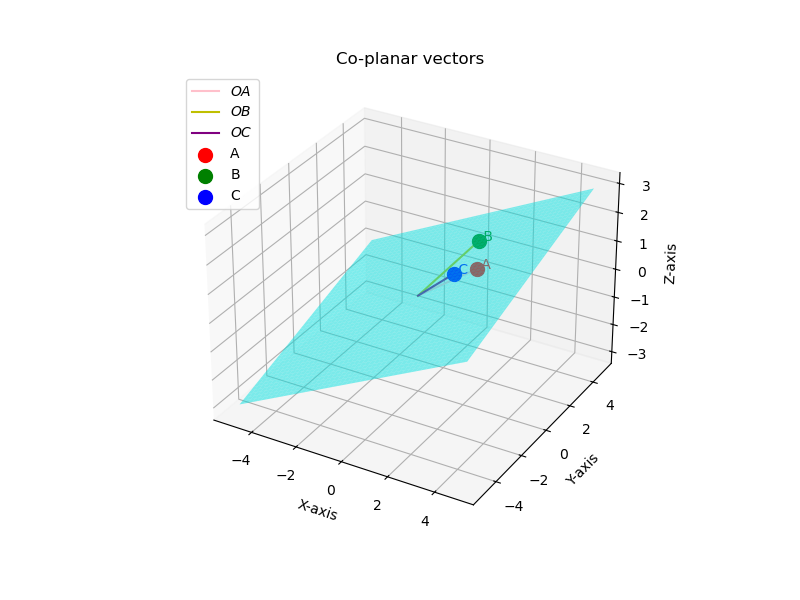
\includegraphics[scale=0.5]{plot}
    \caption{}
    \label{fig:plot}
\end{figure}
\end{document}
